\documentclass[twoside, a4paper, 10pt]{report}
\usepackage[italian]{babel}
\usepackage[utf8]{inputenc}
\usepackage[margin=1in]{geometry}
\usepackage{graphicx}
\usepackage{fancyhdr}
\usepackage{array}
\usepackage{colortbl}
\usepackage{lastpage}
\usepackage{titlesec}
\usepackage{float}
\usepackage{subcaption}
\usepackage{hyperref}
\usepackage{afterpage}
\usepackage{amsmath}

% Ridefinizione per il titolo dei capitoli
\titleformat{\chapter}[hang]{\LARGE\bfseries}{\thechapter}{1em}{} 
\titlespacing{\chapter}{0pt}{0pt}{1em}

% Definizione della path per le immagini
\graphicspath{{../images/}}

% Set the version of the document
\newcommand{\version}{0.2}
\newcommand{\ProjectTitle}{SatisTrento}
\newcommand{\ProjectTitleShort}{satisTrento}
\newcommand{\FileName}{D2-\ProjectTitleShort-analisiProgettazione}

% Definizione dei dati del documento
\title{Analisi e Progettazione - \ProjectTitle}
\author{Facchini Luca, Prigione Luca, Faa Enrico}
\date{A.A. 2024/2025}

% Definizione metadati PDF
\hypersetup{
    pdftitle={\ProjectTitle},
    pdfauthor={Facchini Luca, Prigione Luca, Faa Enrico},
    pdfsubject={Analisi e Progettazione},
    pdfkeywords={\ProjectTitle, Analisi e Progettazione, Comune di Trento, UniTN}
}

% Rimozione scritta "Capitolo" dai titoli dei capitoli
\renewcommand{\chaptermark}[1]{%
    \markboth{
        \thechapter.\ #1%
    }{}%
}
% Definizione del layout della pagina
\fancypagestyle{stdPage}{
    \setlength{\headheight}{24.0pt} 
    \renewcommand{\footrulewidth}{0.4pt}
    \fancyhead{}
    \fancyfoot{}
    \fancyhead[LE,RO]{\begin{tabular}{l l}
        \textbf{Document:} & Analisi e Progettazione \\
        \textbf{Version:} & \version
    \end{tabular}}
    \fancyfoot[LE,RO]{\thepage / \pageref*{LastPage}}
    \fancyhead[LO,RE]{\leftmark}
}
\fancypagestyle{plain}{
    \pagestyle{stdPage}
}
\fancypagestyle{index}{
    \pagestyle{stdPage}
    \fancyfoot[LE,RO]{\thepage}
}

\fancypagestyle{emptyPage}{
    \setlength{\headheight}{24.0pt} 
    \renewcommand{\headrulewidth}{0pt}
    \fancyhead{}
    \fancyfoot{}
}

% Definizione della pagina bianca
\newcommand\blankpage{%
    \null
    \thispagestyle{empty}%
    \addtocounter{page}{-1}%
    \newpage}

\begin{document}
    \pagestyle{fancy}
    \pagenumbering{Roman} 
    
    \begin{titlepage}
        \thispagestyle{emptyPage}
        
\includegraphics[width=0.33\textwidth]{logoUni.png}
        \vspace{1cm}\newline
        \textbf{Progetto:}
        \vspace{0.5cm}
        \begin{center}
            \textbf{\Huge{\ProjectTitle}}
        \end{center}
        \vspace{1cm}
        \textbf{Titolo del documento:}
        \vspace{0.5cm}
        \begin{center}
            \textbf{\huge{Analisi e Progettazione}}
        \end{center}
        \vspace{1cm}
        \textbf{Document Info}
        \vspace{0.5cm}
        % Table with document info
        \begin{center}
            \begin{tabular}{|l|l|l|c|}  
                \hline
                {\cellcolor[rgb]{0,0.502,1}}\textcolor{white}{\textbf{Doc. Name}}   & \FileName & {\cellcolor[rgb]{0,0.502,1}}\begin{tabular}[c]{@{}>{\cellcolor[rgb]{0,0.502,1}}l@{}}\textcolor{white}{\textbf{Doc.}}\\\textcolor{white}{\textbf{Number}}\end{tabular} & D2 V\version  \\ 
                \hline
                {\cellcolor[rgb]{0,0.502,1}}\textcolor{white}{\textbf{Description}} & \multicolumn{3}{l|}{Documento di analisi e progettazzione}\\
                \hline
            \end{tabular}
        \end{center}
        % Document authors (1 per line) with name and ID aligned to the right but with some space from the right border 
        \vspace{1.5in}
        \vfill
        \begin{flushright}
            \rightskip=2cm
            \begin{tabular}{r l}
                \multicolumn{2}{c}{\textbf{Authors}} \\
                Facchini Luca & 245965 \\
                Prigione Luca & 242880 \\
                Faa Enrico & 243889
            \end{tabular}
        \end{flushright}
        \vfill
    \end{titlepage}
    % \afterpage{\blankpage} % Uncomment this line if to print as a booklet
    \begingroup
        \setcounter{tocdepth}{1}
        \tableofcontents
        \thispagestyle{index}
    \endgroup
    \pagestyle{stdPage}
    % \afterpage{\blankpage} % Uncomment this line if to print as a booklet
    \newpage
    \pagenumbering{arabic} 
    
    \chapter{Requisiti Funzionali}
\label{ch:requisitiFunzionali}

Di seguito vengono riportati i requisiti funzionali (\texttt{RF}) del programma "SatisTrento" tramite \textit{Use Case Diagram} (\texttt{UCD}) progettati usando il linguaggio \texttt{UML}.

% Esempio di markup
\section{\underline{Utente non loggato}}
    Di seguito i requisiti associati all'Utente non loggato:
    \begin{itemize}
        \item \textbf{RF1}: Visualizzazione città
        \item \textbf{RF2}: Interazione con la mappa
        \item \textbf{RF3}: Visualizzazione zona
        \item \textbf{RF4}: Elenco strutture
        \item \textbf{RF5}: Multi lingua
        \item \textbf{RF6}: Login
    \end{itemize}
    \begin{figure}[H]
        \centering
        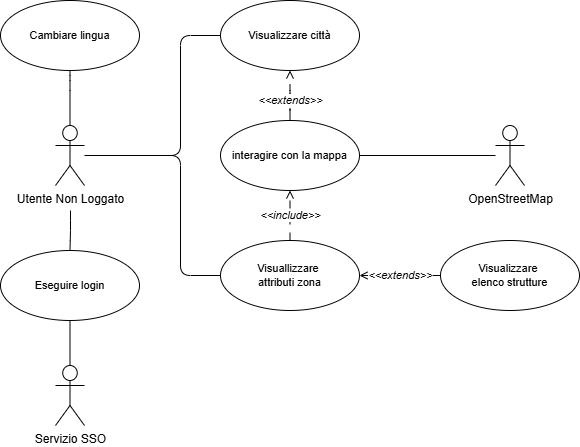
\includegraphics[width=0.8\textwidth]{UseCase_diagrams/NonLoggato.drawio.png}
        \caption{Use Case Diagram dell'Utente non loggato}
    \end{figure}

    \subsection{Visualizzare città}
        \subsubsection{Riassunto}
            Questo Use Case descrive come l'utente può visualizzare gli attributi e la mappa della città
        \subsubsection{Descrizione}
            \begin{itemize}
                \item Il sistema mostra nella parte sinistra dello schermo gli attributi demografici e riguardanti la soddisfazione della città
                \item Il sistema mostra nella parte destra dello schermo la mappa della città suddivisa nella zona selezionata (Estensione 1)
            \end{itemize}
        \subsubsection{Estensioni}
            \begin{itemize}
                \item La tipologia di zona selezionata di default è quella dei quartieri
            \end{itemize}
    
    \subsection{Interagire con la mappa}
        \subsubsection{Riassunto}
            Questo Use Case descrive come l'utente può interagire con la mappa
        \subsubsection{Descrizione}
            \begin{itemize}
                \item L'utente non loggato posiziona il cursone all'interno dello spazio dedicato alla mappa
                \item Se l'utente utilizza la rotella del mouse oppure uno dei pulsanti presenti in uno degli angoli della mappa
                \item Attraverso le funzionalità fornite da OpenStreetMap la mappa ingrandisce o diminuisce la dimensione dello zoom (Eccezione 1)
                \item Se l'utente preme e trascina il cursore
                \item Attraverso le funzionalità fornite da OpenStreetMap la mappa sposta il focus centrale in funzione del cursore (Eccezione 2)
                \item Se l'utente non loggato seleziona una delle zone all'interno della visuale della mappa (Estensione 1)
                \item Il sistema posiziona il focus centrale della mappa al centro della zona selezionata e ne modifica successivamente lo zoom, il colore e lo spessore dei bordi
                \item Il sistema passa successivamente allo UseCase "Visualizzare zona" della sezione scelta
            \end{itemize}
        \subsubsection{Eccezioni}
            \begin{enumerate}
                \item Nel caso in cui l'utente non loggato cercasse di aumentare o diminuire lo zoom oltre ai limiti imposti, il sistema deve bloccare la nuova modifica allo zoom
                \item Nel caso in cui l'utente non loggato cercasse di spostare il focus centrale oltre ai limiti della città, il sistema deve bloccare la nuova modifica allo spostamento del focus centrale
            \end{enumerate}
        \subsubsection{Estensioni}
            \begin{enumerate}
                \item Nel caso in cui l'utente cliccasse su di una zona già selezionata questa riporterebbe allo UseCase "Visualizzare città"
                \item L'utente, selezionando il pulsante presente nell'angolo della mappa, potrà visualizzare un menù a pop-up e successivamente modificare la tipologia di divisione presente all'interno della mappa
            \end{enumerate}
    
    \subsection{Visualizzare zona}
        \subsubsection{Riassunto}
            Questo Use Case descrive come l'utente può visualizzare la zona selezionata della città
        \subsubsection{Descrizione}
            \begin{enumerate}
                \item Dopo aver interagito con la mappa ed aver selezionato una zona
                \item Il sistema mostra nella parte sinistra dello schermo la mappa centrata sul centro della zona selezionata
                \item Il sistema mostra nella parte destra dello schermo gli attributi demografici e riguardanti la soddisfazione della zona della città selezionata
            \end{enumerate}

    \subsection{Visualizzare elenco strutture}
        \subsubsection{Riassunto}
            Questo Use Case descrive come l'utente può accedere e visualizzare l'elenco delle strutture che forniscono un servizio al cittadino
        \subsubsection{Descrizione}
            \begin{enumerate}
                \item L'utente non loggato preme uno degli attributi presenti a schermo (Eccezione 1)
                \item Il sistema presenta a schermo, ove prima erano presenti gli attributi riguardanti la zona selezionata, una tabella contenente una lista numerata di strutture che offrono il servizio selezionato in precedenza
                \item Il sistema deve successivamente segnalare sulla mappa la posizione delle varie strutture, attraverso un segnalino contenente il numero identificativo presente in tabella della struttura
            \end{enumerate}
        \subsubsection{Eccezioni}
            \begin{enumerate}
                \item Nel caso in cui per una tipologia di dato non fossero presenti strutture il sistema non deve fare nulla
            \end{enumerate}
        \subsubsection{Estensioni}
            \begin{enumerate}
                \item Nel caso in cui l'utente cliccasse il pulante per chiudere la tabella il sistema tornerà alla visualizzazione della zona selezionata in precedenza
            \end{enumerate}

    \subsection{Cambiare lingua}
        \subsubsection{Riassunto}
            Questo Use Case descrive come l'utente può cambiare la lingua dei vari testi presenti nel programma
        \subsubsection{Descrizione}
            \begin{enumerate}
                \item L'utente preme sul menù a tendina presente nella header e seleziona la sezione riguardante la modifica della lingua
                \item Il sistema presenterà a schermo un menù pop-up contenente la lista di lingue per le quali è disponibile la traduzione
                \item Se l'utente seleziona la lingua e clicca il pulsante di conferma (Eccezione 1 e 2)
                \item Il sistema ricarica la pagina selezionata con i testi nella lingua selezionata
            \end{enumerate}
        \subsubsection{Eccezioni}
            \begin{enumerate}
                \item Nel caso in cui l'utente non loggato selezionasse e confermasse la lingua già selezionata, il sistema deve chiudere il pop-up senza apportare alcuna modifica
            \end{enumerate}

    \subsection{Eseguire login}
        \subsubsection{Riassunto}
            Questo Use Case descrive come l'utente non loggato può eseguire il login
        \subsubsection{Descrizione}
            \begin{enumerate}
                \item L'utente preme sul menù a tendina presente all'interno della header e seleziona la sezione riguardante il login
                \item Il sistema reindirizza l'utente alla pagina del service provider della provincia di Trento dal quale potrà accedere al login tramite sistema SSO
                \item Il sistema SSO verifica l'identità dell'utente in questione e la ritorna al sistema (Eccezione 1)
                \item Il sistema controlla che per l'identità certificata dal sistema SSO esista un'account collegato (Eccezione 1)
                \item Il sistema assegna dunque un'identità all'utente assegnandogli il ruolo di proprietà
                \item Il sistema successivamente al login sostituisce l'icona del login con l'immagine profilo dell'account al quale si ha fatto l'accesso e reindirizza l'utente allo UseCase "visualizzare città"
            \end{enumerate}
        \subsubsection{Eccezioni}
            \begin{enumerate}
                \item Nel caso in cui l'autenticazione fallisse o non vi fossero account collegati il sistema ritorna alla pagina dalla quale si ha provato a fare il login
            \end{enumerate}


\section{\underline{Utente Sondaggista}}
    Di seguito i requisiti associati all'Utente Sondaggista:
    \begin{itemize}
        \item \textbf{RF7}: Logout
        \item \textbf{RF8}: Visualizzazione sondaggi
        \item \textbf{RF9}: Gestione sondaggi
        \item \textbf{RF10}: Visualizzazione voti
        \item \textbf{RF11}: Gestione voti
    \end{itemize}
    \begin{figure}[H]
        \centering
        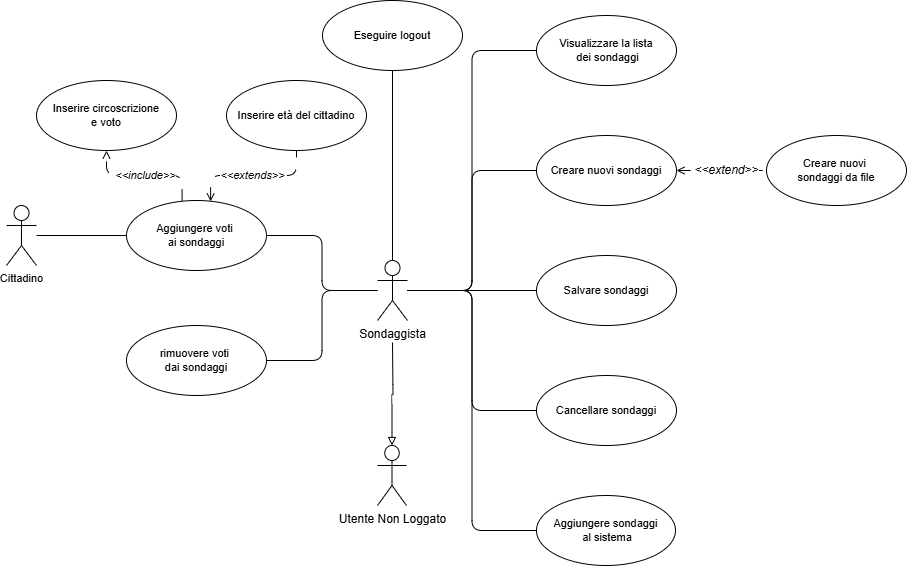
\includegraphics[width=0.8\textwidth]{UseCase_diagrams/Sondaggista.drawio.png}
        \caption{Use Case Diagram dell'Utente sondaggista}
    \end{figure}

    \subsection{Logout}
        \subsubsection{Riassunto}
            Questo Use Case descrive come l'utente può fare logout
        \subsubsection{Descrizione}
            \begin{enumerate}
                \item L'utente sondaggista preme sul menù a tendina presente all'interno della header e seleziona la sezione riguardante il logout
                \item Il sistema scollega lo user dall'account al quale era collegato riportandolo allo stato di utente non loggato, infine 
                ricarica la pagina riportando l'utente alla 'visualizzazione città'
            \end{enumerate}

    \subsection{Visualizzare i sondaggisti}
        \subsubsection{Titolo}
            Questo Use Case descrive come l'utente sondaggista visualizzerà i sondaggi e le interfacce per gestirli
        \subsubsection{Descrizione}
            \begin{enumerate}
                \item Il sistema mostra nel riquadro in alto a sinistra dello schermo l'interfaccia per la creazione di nuovi sondaggi con relative caselle di testo e pulsante per la creazione
                \item Il sistema mostra nel riquadro in basso a sinistra dello schermo l'interfaccia per il caricamento dei sondaggi attraverso pulsante o "drag and drop"
                \item Il sistema mostra nel riquadro in alto a destra dello schermo l'elenco dei sondaggi non ancora caricati, o in fase di caricamento, a sistema con relativo stato della sessione (Eccezione 1)
                \item Il sistema mostra nel riquadro in basso a destra dello schermo l'elenco dei sondaggi già caricati a sistema con relativo stato di caricamento e stato di verifica dei dati inseriti (Eccezione 1)
            \end{enumerate}
        \subsubsection{Eccezioni}
            \begin{enumerate}
                \item Nel caso in cui non fossero presenti sondaggi all'interno di uno degli elenchi il sistema mostrerà a schermo un messaggio per avvisare che tale sezione risulta vuota
            \end{enumerate}

    \subsection{Gestione sonaggi}

    \subsection{Visualizzare i voti}
        \subsubsection{Titolo}
            Questo Use Case descrive come l'utente sondaggista visualizzerà i voti e le interfacce per gestirli
        \subsubsection{Descrizione}
            \begin{enumerate}
                \item Il sistema mostra nella parte sinistra dello schermo un riassunto del numero di voti presenti all'interno del sondaggio e in basso una tabella riassuntiva riguardante il numero di voti ricevuti per quartiere
                \item Il sistema mostra nel riquadro in alto a destra dello schermo l'interfaccia per il caricamento dei voti con le corrispettive caselle di testo
                \item Il sistema mostra nel riquadro in basso a destra dello schermo l'interfaccia per la gestione dei sondaggi
                \item Il sistema mostra nel riquadro in basso al centro dello schermo l'elenco dei voti caricati in precedenza, su ogni voto è inoltre presente l'id, l'ora al quale è stato caricato il voto e infine il pulsante per eliminarlo (Eccezione 1)
            \end{enumerate}
        \subsubsection{Eccezioni}
            \begin{enumerate}
                \item Nel caso in cui non fossero presenti voti all'interno della lista il sistema mostrerà a schermo un messaggio per avvisare che tale sezione risulta vuota
            \end{enumerate}

    \subsection{Gestione voti}
    
    \chapter{Analisi dei componenti}
    Nel presente capitolo viene presentata l'architettura in termini di componenti (CMP) interni al sistema definiti sulla base dei requisiti analizzati in precedenza.

\section{Definizione dei componenti}
    Definiamo di seguito i componenti del sistema con le relative funzionalità.
    
    \subsection{\texttt{CMP1}: Gestione grafici}
        \subsubsection{Descrizione} 
            Il componente si occupa della funzionalità di generare per ogni attributo un grafico storico. Tale grafico raffigura l'andamento del relativo attributo in un dato arco di tempo.
        \subsubsection{Interfaccia richiesta - Selezione attributo:}
            viene richiesta al \textit{CMP} ``Gestione Attributi'' la selezione dell'attributo per il quale è necessario generare un grafico.
        \subsubsection{Interfaccia richiesta - Attributi:}
            nella seguente interfaccia vengono richiesti al \textit{CMP} ``Gestione Database'' i dati riguardanti l'attributo di interesse.
        \subsubsection{Interfaccia fornita - Grafico:}
            il componente fornisce dunque il grafico raffigurante l'andamento nel tempo dell'attributo fornito.
    
    \subsection{\texttt{CMP2}: Gestione lingua}
        \subsubsection{Descrizione} 
            Il componente si occupa della funzionalità di generare in base alla lingua selezionata il testo presente nella pagina basandosi sui testi presenti all'interno di file JSON appositi.
        \subsubsection{Interfaccia richiesta - Selezione lingua:}
            viene richiesta la selezione da parte dell'utente della lingua di preferenza.
            In caso di default la lingua selezionata sarà l'italiano.
        \subsubsection{Interfaccia fornita - Testo:}
            il componente fornisce il testo necessario tradotto in base alla lingua selezionata in precedenza.

    \subsection{\texttt{CMP3}: Gestione mappa e tabella}
        \subsubsection{Descrizione}
            Il componente si occcupa di fornire all'utente una rappresentazione dettagliata della città e delle suoi zone geografiche. Attraverso il seguente componente è inoltre possibile selezionare una delle zone geografiche per la quali si vuole ricevere maggiori informazioni. 
        \subsubsection{Interfaccia richiesta - Selezione zona:}
            attraverso la seguente interfaccia il componente riceve dall'utente la zona geografica sulla quale vuole ricevere maggiori informazioni. Nel caso in cui non vi fosse una zona selezionata verrà utilizzata quella di default, ovvero l'intero comune.
        \subsubsection{Interfaccia richiesta - Testo:}
            il testo comprende la traduzione dei dati forniti e dei nomi presenti nelle varie aree geografiche.
        \subsubsection{Interfaccia richiesta - Mappa di trento:}
            fa una richiesta a OpenStreetMap per avere la mappa del comune.
        \subsubsection{Interfaccia fornita - Immagine:}
            rappresentazione grafica tramite mappa della città o dell'area geografica selezionata.
        \subsubsection{Interfaccia fornita - Zona selezionata:}
            indica agli altri componenti la zona selezionata sulla quale andranno effettuate, nel caso in cui si possedessero le autorizzazioni necessarie, le seguenti operazioni.
    
    \subsection{\texttt{CMP4}: Gestione attributi}
        \subsubsection{Descrizione}
            Il componente si occupa di fornire all'utente tutte le informazioni necessarie riguardo le zone geografiche o i servizi presenti all'interno di esse. Il seguente componente è dunque in grado di generare diverse rappresentazioni degli attributi in base alle autorizzazioni, alla zona o al servizio selezionato che arrivano in ingresso alle varie interfacce richieste.
        \subsubsection{Interfaccia richiesta - Testo:}
            il testo comprende la traduzione dei vari attributi, servizi e delle categorie di attributi presenti all'interno delle varie rappresentazioni degli attributi.
        \subsubsection{Interfaccia richiesta - Zona selezionata:}
            indica la zona per la quale bisogna visualizzare gli attributi principali. Nel caso in cui non vi fosse una zona selezionata verrà utilizzata quella di default, ovvero l'intero comune.
        \subsubsection{Interfaccia richiesta - Servizio selezionato:}
            indica l'attributo per il quale bisogna visualizzare la lista dei servizi che svolgono un ruolo attivo, all'interno della zona selezionata, all'interno dell'ambito di tale attributo. Nel caso in cui non vi fosse un'attributo selezionato verrà utilizzata quella di default, ovvero nessun attributo.
        \subsubsection{Interfaccia richiesta - Autorizzazione:}
            bit che segnala se l'utente ha il permesso necessario per compiere o meno un'azione.
        \subsubsection{Interfaccia richiesta - Attributi:}
            nella seguente interfaccia vengono richiesti al \textit{CMP} ``Gestione Database'' gli attributi di  interesse.
        \subsubsection{Interfaccia fornita - Selezione attributo:}
            fornisce al \textit{CMP} ``Gestione Grafici'' gli attributi per i quali è necessario fornire la rappresentazione di un grafico per uno studio ulteriore dell'andamento.
        \subsubsection{Interfaccia fornita - Valore attributi:}
            l'interfaccia fornisce una rappresentazione degli attributi presenti in base ai dati forniti all'interno delle interfacce richieste.

    \subsection{\texttt{CMP5}: Gestione database}
        \subsubsection{Descrizione} 
            il componente si occupa di fornire la raccolta dei dati più importanti. Salva nel database tutti i dati relativi alle categorie e agli attributi stessi, tiene inoltre traccia dei voti e integra ciò con i voti presenti all'interno dei sondaggi valutati positivamente.
        \subsubsection{Interfaccia richiesta - Dati database:}
            raccolta di tutti i dati presenti all'interno del database, questi dati riguardano gli attributi per il \textit{CMP} ``Gestione Attributi'' e i voti per i vari \textit{CMP} correlati.
        \subsubsection{Interfaccia richiesta - Dati strutture modificati:}
            raccolta dei dati appartenenti ad una struttura che ha appena subito una modifica.
        \subsubsection{Interfaccia richiesta - Cancellazione sondaggio:}
            codice identificativo che permette la rimozione di un sondaggio e di tutti i voti collegati al corrispettivo sondaggio dal database.
        \subsubsection{Interfaccia richiesta - Sondaggi approvati:}
            codice identificativo che permette l'aggiunta di un sondaggio all'interno della lista di sondaggi accettati e l'aggiunta di tutti i voti collegati al corrispettivo sondaggio.
        \subsubsection{Interfaccia fornita - Attributi:}
            il componente fornisce l'insieme degli attributi presenti all'interno del database che verranno filtrati nei successivi \textit{CMP}.
        \subsubsection{Interfaccia fornita - Modifiche databse:}
            raccolta di tutti i dati che sono stati modificati e che vanno dunque sostituiti all'interno della base di dati.
    
    \subsection{\texttt{CMP6}: Gestione dati strutture}
        \subsubsection{Descrizione}
            il componente si occupa di permettere agli utenti che ne hanno l'autorizzazione di poter gestire i dati sui quali possono esercitare il controllo.
        \subsubsection{Interfaccia richiesta - Autorizzazione:}
            bit che segnala se l'utente ha il permesso necessario per compiere o meno un'azione.
        \subsubsection{Interfaccia richiesta - Modifica dei dati:}
            dati appartenenti ad una struttura i quali, in seguito, verranno inviati al database per poter essere modificati.
        \subsubsection{Interfaccia fornita - Dati strutture modificati:}
            insieme dei dati appartenenti alla struttura che ha appena subito una modifica da un'utente autorizzato a compiere tale operazione.

    \subsection{\texttt{CMP7}: Gestione invio richieste}
        \subsubsection{Descrizione}
            il componente si occupa di inviare le richieste, fornite da utenti con le corrispettive autorizzazioni, al \textit{CMP} ``Gestione invio risposte'' e di gestire la corrispettiva risposta. Le richieste permetteranno di mettere in contatto diretto le circoscrizioni e il comune permettendo una comunicazione più efficente.
        \subsubsection{Interfaccia richiesta - Testo richiesta:}
            rappresenta il testo completo della richiesta fornito dalla circoscrizione.
        \subsubsection{Interfaccia richiesta - Risposte:}
            racchiude il testo completo della risposta fornito dal comune e il codice identificativo della richiesta alla quale il messaggio sta rispondendo.
        \subsubsection{Interfaccia richiesta - Autorizzazione:}
            bit che segnala se l'utente ha il permesso necessario per compiere o meno un'azione.
        \subsubsection{Interfaccia fornita -T esto risposte:}
            racchiude il testo completo della richiesta fornito dalla circoscrizione con in coda il testo completo della risposta contrassegnato dall'utente che ha risposto.
        \subsubsection{Interfaccia fornita - Richieste:}
            rappresenta il testo completo della richiesta, il codice identificativo della richiesta, il codice identificativo della circoscrizione ed il codice identificativo dell'utente che ha inviato la richiesta.

    \subsection{\texttt{CMP8}: Gestione invio risposte}
        \subsubsection{Descrizione}
            il componente si occupa di fornire le risposte per le richieste inviate dal \textit{CMP} ``Gestione invio risposte''. Le risposte permetteranno di semplificare la comunicazione diretta tra le circoscrizioni ed il comune stesso basandosi su di un servizio più efficente.
        \subsubsection{Interfaccia richiesta - Richieste:}
            rappresenta il testo completo della richiesta, il codice identificativo della richiesta, il codice identificativo della circoscrizione ed il codice identificativo dell'utente che ha inviato la richiesta.
        \subsubsection{Interfaccia richiesta - Testo risposta:}
            rappresenta il testo completo della risposta fornito dal comune.
        \subsubsection{Interfaccia richiesta - Autorizzazione:}
            bit che segnala se l'utente ha il permesso necessario per compiere o meno un'azione.
        \subsubsection{Interfaccia fornita - Risposte:}
            racchiude il testo completo della risposta fornito dal comune e il codice identificativo della richiesta alla quale il messaggio sta rispondendo.
        \subsubsection{Interfaccia fornita - Testo richieste:}
            rappresenta il testo completo della richiesta, il nome della circoscrizione ed il nome dell'utente che ha inviato la richiesta.

    \subsection{\texttt{CMP9}: Gestione voti}
        \subsubsection{Descrizione}
            il componente si occupa di permettere ai sondaggisti di aggiungere o eliminare i voti. Nel momento di aggiunta del voto oltre al valore del voto devono anche essere inserite una serie di informazioni base del cittadino votante.
        \subsubsection{Interfaccia richiesta - Autorizzazione:}
            bit che segnala se l'utente ha il permesso necessario per compiere o meno un'azione.
        \subsubsection{Interfaccia richiesta - Informazioni cittadino:}
            insieme dei dati riguardanti l'età e il quartiere di provenienza del cittadino votante.
        \subsubsection{Interfaccia richiesta - Valore voto:}
            valore numerico che rappresenta il grado di soddisfazione del cittadino.
        \subsubsection{Interfaccia fornita - Voti:}
            insieme di informazioni che racchiude l'insieme dei voti e delle informazioni generiche riguardanti i cittadini che hanno votato.

    \subsection{\texttt{CMP10}: Gestione sondaggi}
        \subsubsection{Descrizione}
            il componente si occupa di permettere ai sondaggisti di modificare, aggiungere, completare o eliminare i sondaggi. Nel momento in cui un sondaggio viene eliminato tale informazione viene propagata anche al \textit{CMP} ``Gestione database''. Nel momento in cui un sondaggio viene completato il sondaggio viene inviato al \textit{CMP} ``approvazione sondaggi'' in modo che possa venire valutato dagli utenti amministratore.
        \subsubsection{Interfaccia richiesta - Voti:}
            insieme di informazioni che racchiude l'insieme dei voti e delle informazioni generiche riguardanti i cittadini che hanno votato.
        \subsubsection{Interfaccia richiesta - Autorizzazione:}
            bit che segnala se l'utente ha il permesso necessario per compiere o meno un'azione.
        \subsubsection{Interfaccia fornita - Sondaggi completati:}
            insieme delle informazioni formato dall'insieme dei voti, l'insieme delle informazioni generiche riguardanti i cittadini che hanno votato e il codice identificativo del sondaggista.
        \subsubsection{Interfaccia fornita - Cancellazione sondaggio:}
            codice identificativo che permette la rimozione di un sondaggio e di tutti i voti collegati al corrispettivo sondaggio dal database.

    \subsection{\texttt{CMP11}: Gestione approvazione sondaggi}
        \subsubsection{Descrizione}
            il componente si occupa di permettere agli utenti amministratore di monitorare i sondaggi contrassegnati come completati prima che questi possano venire caricati a sistema. Tale processo permette agli utenti amministratori di controllare da come e da chi sono stati eseguiti i sondaggi, permettendo loro di monitorare a priori i dati che vengono inviati all'interno del database. 
        \subsubsection{Interfaccia richiesta - Sondaggi completati:}
            insieme delle informazioni formato dall'insieme dei voti, l'insieme delle informazioni generiche riguardanti i cittadini che hanno votato e il codice identificativo del sondaggista.
        \subsubsection{Interfaccia richiesta - Autorizzazione:}
            bit che segnala se l'utente ha il permesso necessario per compiere o meno un'azione.
        \subsubsection{Interfaccia richiesta - Approvazione:}
            viene richiesto all'utente amministratore di selezionare se il sondaggio è pronto o meno per essere caricato all'interno del database.
        \subsubsection{Interfaccia fornita - Sondaggi approvati:}
            codice identificativo che permette l'aggiunta di un sondaggio all'interno della lista di sondaggi accettati e l'aggiunta di tutti i voti collegati al corrispettivo sondaggio.
    
    \subsection{\texttt{CMP12}: Gestione ruoli utente}
        \subsubsection{Descrizione}
            il componente si occupa di aggiungere, rimuovere o modificare i ruoli dei vari utenti. Tale funzionalità permette di aggiungere o rimuovere le funzionalità alle quali un'utente può avere accesso. 
        \subsubsection{Interfaccia richiesta - Codice fiscale:}
            si tratta del codice identificativo attraverso il quale il componente riesce a selezionare l'utente che subirà le modifiche ai ruoli.
        \subsubsection{Interfaccia richiesta - Tipologia di ruolo:}
            codice identificativo del ruolo che si vuole andare ad aggiungere/rimuovere.
        \subsubsection{Interfaccia richiesta - Autorizzazione:}
            bit che segnala se l'utente ha il permesso necessario per compiere o meno un'azione.
        \subsubsection{Interfaccia fornita - Ruoli utenti:}
            insieme delle informazioni che determinano a quali ruoli sono autorizzati i diversi utenti all'interno del programma.

    \subsection{\texttt{CMP13}: Gestione autenticazione}
        \subsubsection{Descrizione}
            il componente si occupa di verificare l'identità dell'utente che sta effettuando l'accesso all'interno del sistema. Il componente si basa su un sistema di autenticazione SSO attraverso il quale è in grado di fornire all'utente l'accesso al corrispettivo ruolo. Tale componente include le funzionalità di login e di logout.
        \subsubsection{Interfaccia richiesta - Autenticazione utente SSO:}
            autorizzazione all'accesso al sistema preveniente dall'SSO che, previo controllo delle credenziali inserite dall'utente, conferma che tali credenziali sono corrette. Confermando dunque l'identità dell'utente.
        \subsubsection{Interfaccia richiesta - Richiesta di login:}
            richiesta da parte dell'utente di poter essere reindirizzato al sistema SSO di preferenza per poter accedere ad alcune funzionalità.
        \subsubsection{Interfaccia richiesta - Richiesta di logout:}
            richiesta da parte dell'utente di poter essere scollegato dal ruolo al quale l'utente è temporaneamente connesso, riportando così l'utente al ruolo di ``Utente non loggato''.
        \subsubsection{Interfaccia fornita - Richiesta a servizi SSO:}
            reindirizzamento dell'utente verso il sistema SSO scelto per l'inserimento delle proprie credenziali.
        \subsubsection{Interfaccia fornita - Autenticazione:}
        codice univoco che identifica il ruolo che l'utente ha all'interno del programma, ovvero l'insieme delle funzioanlità alle quali le divese tipologie di utenti hanno accesso.
    
    \subsection{\texttt{CMP14}: Gestione autorizzazioni}
        \subsubsection{Descrizione}
            il componente si occupa di gestire i vari diritti e privilegi che hanno i diversi utenti in base al ruolo che questi hanno. Questo componente richiede le informazioni sui ruoli degli utenti e il ruolo fornito dall'autorizzazione e in base a ciò determina a quali funzionalità questo utente può avere accesso. 
        \subsubsection{Interfaccia richiesta - Ruoli utenti:}
            insieme delle informazioni che determinano a quali ruoli sono autorizzati i diversi utenti all'interno del programma.
        \subsubsection{Interfaccia richiesta - Autenticazione:}
            codice univoco che identifica il ruolo che l'utente ha all'interno del programma, ovvero l'insieme delle funzioanlità alle quali le divese tipologie di utenti hanno accesso.
        \subsubsection{Interfaccia fornita - Autorizzazione:}
            insieme di bit in uscita che determinano se l'utente ha il permesso necessario per compiere o meno un'azione.

\section{Diagramma dei componenti}
    Viene riportato di seguito un diagramma complessivo di tutti i componenti di sistema e le loro interconnessioni descritte in precedenza.
    \begin{figure}[H]
        \centering
        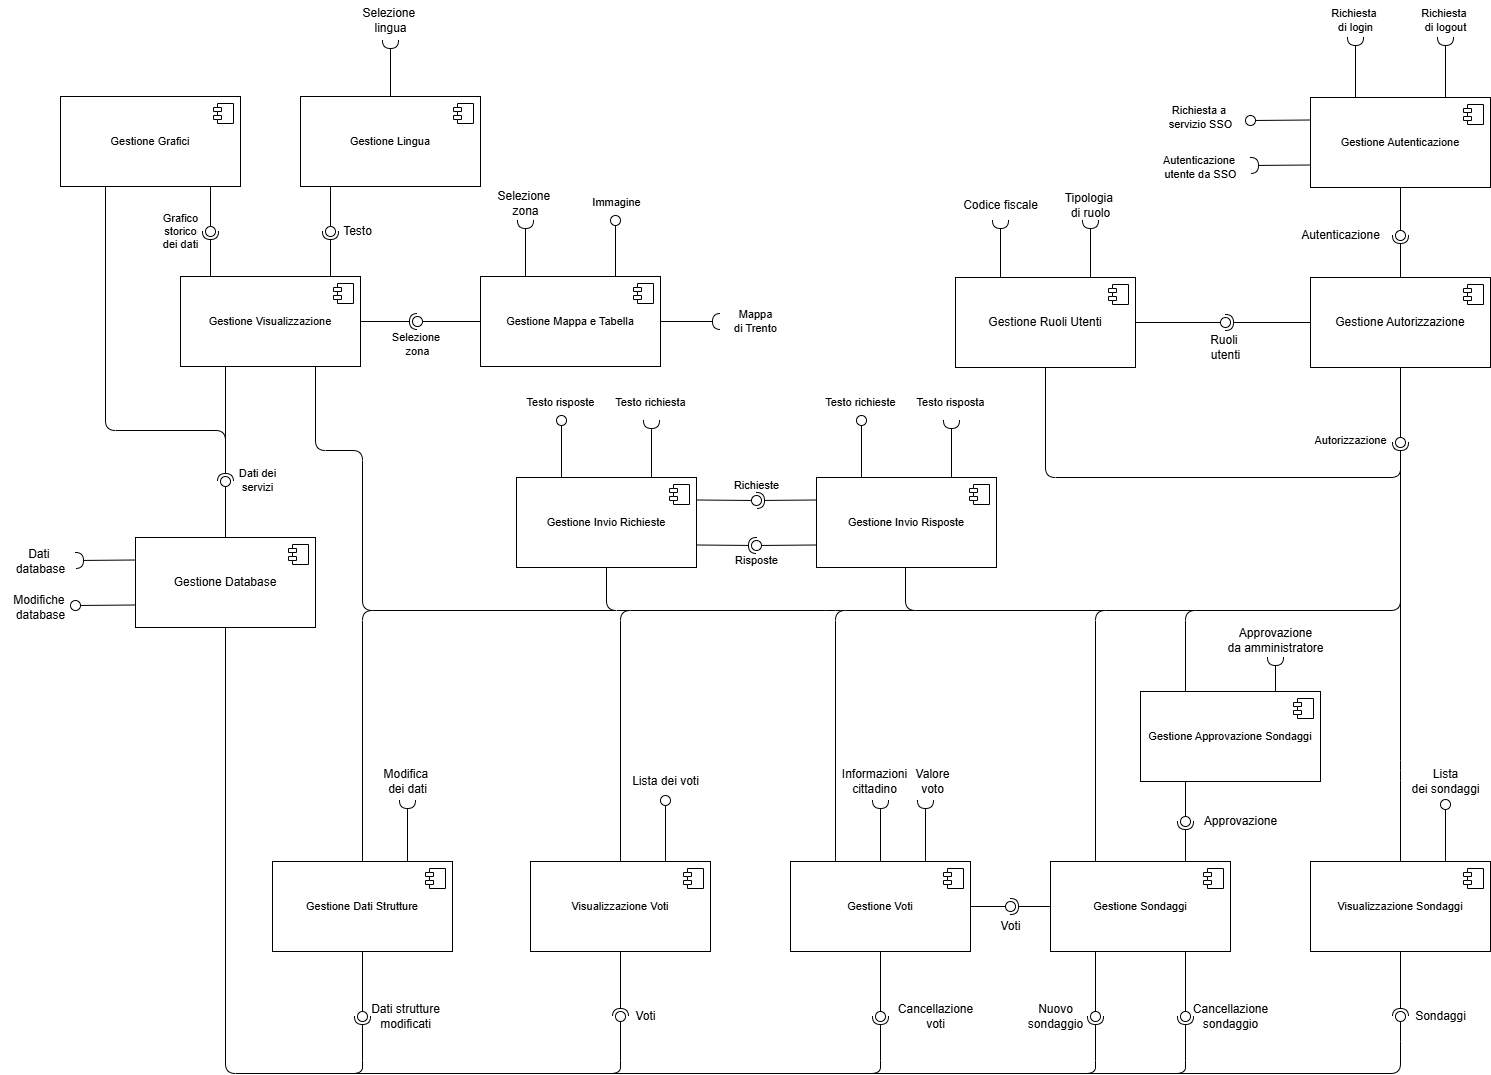
\includegraphics[width=1\textwidth]{ComponentDiagrams/ComponentDiagram.drawio.png}
    \end{figure}

    \chapter{Diagramma delle classi}

\section{Definizione delle classi}

    \subsection*{1. Utente}
        L'attore utente, da cui la classe omonima, rappresenta la classe astratta che viene estesa da tutte le tipologie di utenti presenti all'interno del programma. All'interno della classe ``Utente'' sono presenti i campi contenenti le informazioni personali ed i metodi comuni a tutti gli utenti, oppure necessari per definire il ruolo che l'utente ricopre all'interno del programma stesso.

    \subsection*{2. Utente\_Analista}
        La classe ``Utente\_Analista'' raffigura la classe di utenti che hanno la possibilità di visualizzare una maggiore quantità di informazioni e di statistiche al fine di analizzarne l'andamento e di studiare le strategie più efficaci per aumentare il grado di soddisfazione dei cittadini all'interno della città. La classe estende la classe ``Utente'', alla quale aggiunge gli attributi e i metodi necessari per gestire l'area di influenza dell'Analista stesso.

    \subsection*{3. Utente\_Sondaggista}
        La classe ``Utente\_Sondaggista'' raffigura la classe di utenti che hanno la possibilità di aggiungere o eliminare i sondaggi ed i voti presenti all'interno dei sondaggi stessi, permettendo ai cittadini la possibilità di esprimere il proprio grado di soddisfazione riguardo i servizi comunali e le politiche attutate dal comune. La classe estende la classe ``Utente'', alla quale aggiunge gli attributi e i metodi necessari per gestire i sondaggi, i voti e l'area di influenza del sondaggista stesso.

    \subsection*{4. Utente\_Circoscrizione}
        La classe ``Utente\_Circoscrizione'' raffigura la classe di utenti che hanno la possibilità di gestire le funzionalità di maggiore rilievo all'interno della circoscrizione di appartenenza, tra le quali la gestione delle strutture, dei ruoli e delle richieste. La classe estende la classe ``Utente'', alla quale aggiunge gli attributi e i metodi necessari per le funzionalità di gestione delle strutture, dei ruoli e delle richieste.

    \subsection*{5. Utente\_Amministratore}
        La classe ``Utente\_Amministratore'' raffigura la classe di utenti che hanno la possibilità di gestire le funzionalità di maggiore rilievo all'interno del comune di appartenenza, tra le quali la gestione delle strutture, dei ruoli, dell'approvazione dei sondaggi e delle risposte alle richieste da parte delle circoscrizioni. La classe estende la classe ``Utente'', alla quale aggiunge gli attributi e i metodi necessari per le funzionalità di gestione delle strutture, dei ruoli e delle risposte.

    \subsection*{6. Richiesta}
        La gestione delle richieste è identificata dalla classe omonima ``Richiesta'', tale classe permette di gestire il testo della richiesta, le informazioni riguardanti il mittente e la risposta fornita da uno degli utenti amministratore. Una volta completati i campi della richiesta e inviata la richiesta agli utenti amministratore la classe aspetterà una risposta da poter fornire all'utente circoscrizione da parte della classe ``Risposta''.
    
    \subsection*{7. Risposta}
        La gestione delle risposte è identificata dalla classe omonima ``Risposta'', tale classe permette di gestire la richiesta da parte dell'utente circoscrizione e il testo della relativa risposta. Una volta ricevuta la richiesta l'utente amministratore è in grado di fornire un relativo testo di risposta e successivamente inviare la risposta al mittente presente nella classe la classe ``Richiesta''.

    \subsection*{8. Sondaggio}
        Per la gestione dei sondaggi è stata identificata la classe omonima ``Sondaggio'', tale classe permette di gestire le informazioni che vengono caricare all'interno del sondaggio e le operazioni che vengono effettuate sul sondaggio stesso. L'utente sondaggista crea il sondaggio, successivamente sui sondaggi aperti sarà possibile aggiungere e rimuovere i voti, infine, successivamente alla chiusura del sondaggio, sarà possibile per gli utenti sondaggisti approvare o rifiutare i sondaggi stessi.
    
    \subsection*{9. Voto}
        I voti presenti all'interno della classe ``Sondaggi'' sono appartenenti alla classe ``Voto'', tale classe ha lo scopo di memorizzare i dati generici, quali la circoscrizione di appartenenza e la fascia d'età, dei cittadini votanti oltre che il voto espresso attraverso un valore numerico.

    \subsection*{10. Zona}
        La classe ``Zona'' rappresenta la classe astratta che viene estesa dalle diverse tipologie di zone geografiche che dividono la città, ovvero quartieri e circoscrizioni. All'interno della classe ``Zona'' sono presenti i campi contenenti le informazioni necessarie per distinguere e memorizzare le diverse zone geografiche oltre ai metodi necessari per gestire le strutture presenti all'interno dell'area geografica e per modificare alcuni dei campi presenti al suo interno.

    \subsection*{11. Circoscrizione}
        La classe ``Circoscrizione'' estende la classe ``Zona'' in quanto questa definisce una zona di territorio specifica, la circoscrizione si compone, oltre che dai campi e dai metodi dalla classe padre, del campo ``Quartieri'' che tiene traccia delle classi ``Quartiere'' dalle quali questa è composta.
    
    \subsection*{12. Quartiere}
        La classe ``Quartiere'' estende la classe ``Zona'' in quanto questa definisce una zona di territorio specifica, il quartiere si compone, oltre che dai campi e dai metodi dalla classe padre, dai metodi necessari per modificare i campi presenti al suo interno.
    
    \subsection*{13. Struttura}
        Per la gestione delle strutture è stata identificata la classe ``Struttura'' che servirà a gestire le informazioni riguardo alle strutture presenti all'interno delle diverse zone geografiche.

\newpage
\section{Diagramma delle classi complessivo}
    Riportiamo di seguito il diagramma delle classi con tutte le classi fino ad ora presentate.
    \begin{figure}[H]
        \centering
        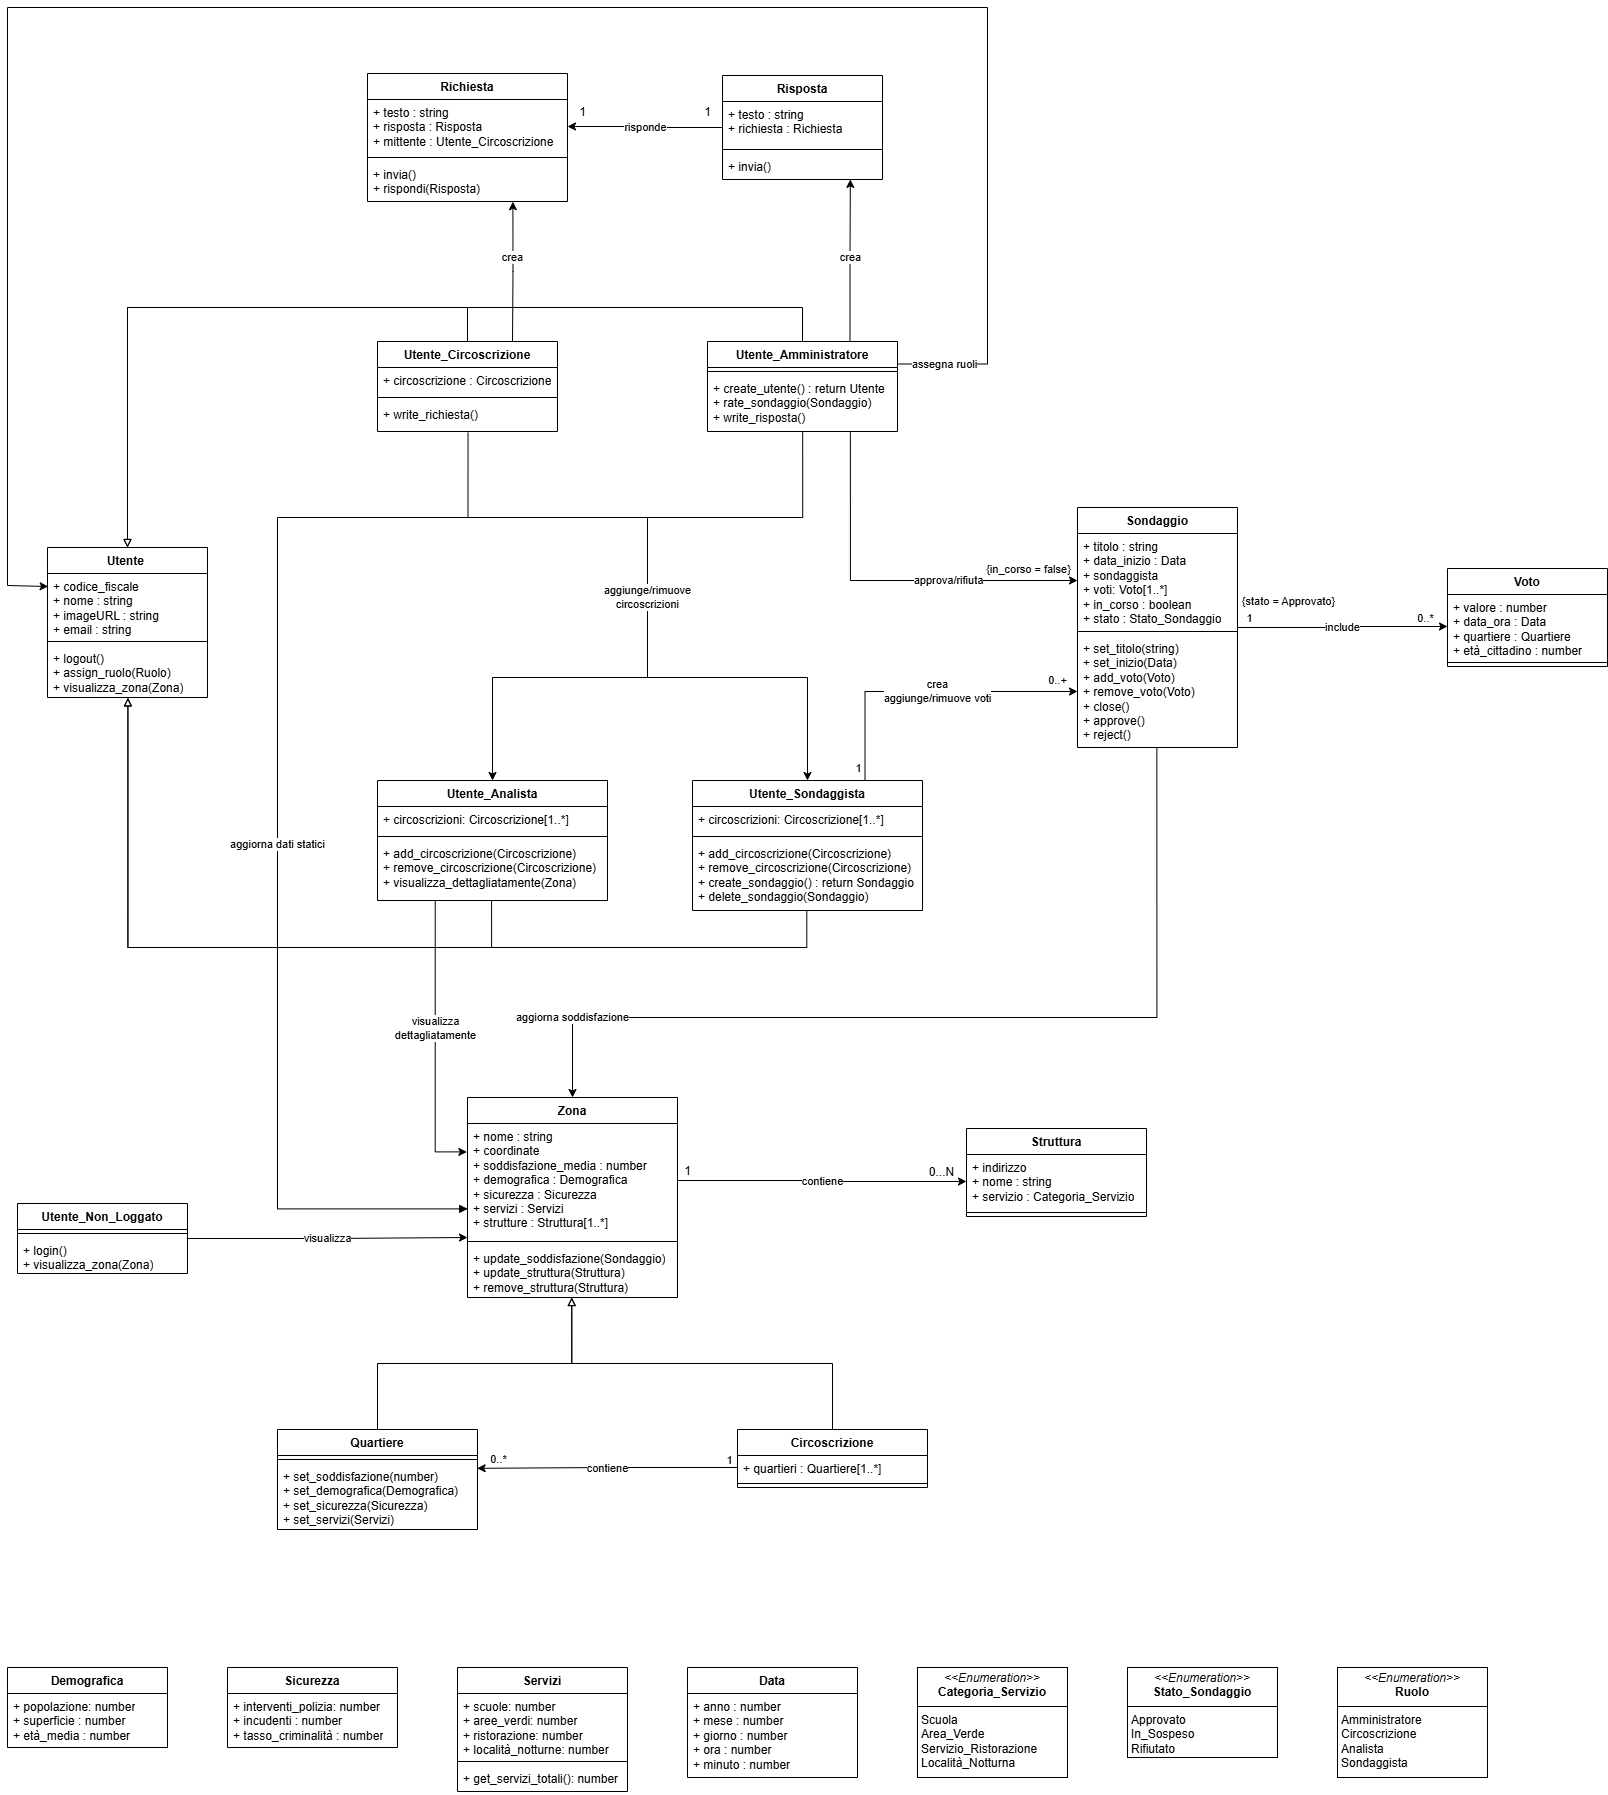
\includegraphics[width=1\textwidth]{ClassDiagram/ClassDiagram.drawio.png}
    \end{figure}
    
    \chapter{Dal Class Diagram alle API}
Riportiamo di seguito una tabella con la mappatura tra i metodi presenti nel diagramma delle classi del capitolo precedente e le API individuate nel documento D3.

{\footnotesize
    \begin{xltabular}{\textwidth}{|l|X|X|X|X|X|}

        \hline \multicolumn{1}{|l|}{\textbf{Classe}} & \multicolumn{1}{X|}{\textbf{Metodo}} & \multicolumn{1}{X|}{\textbf{HTTP Method}} & \multicolumn{1}{X|}{\textbf{URL + Params}} & \multicolumn{1}{X|}{\textbf{Request}} & \multicolumn{1}{X|}{\textbf{Response}} \\ \hline 
        \endfirsthead
        
        \multicolumn{6}{l}%
        {Tabella continuata dalla pagina precedente} \\
        \hline \multicolumn{1}{|l|}{\textbf{Classe}} & \multicolumn{1}{X|}{\textbf{Metodo}} & \multicolumn{1}{X|}{\textbf{HTTP Method}} & \multicolumn{1}{X|}{\textbf{URL + Params}} & \multicolumn{1}{X|}{\textbf{Request}} & \multicolumn{1}{X|}{\textbf{Response}} \\ \hline 
        \endhead
        
        \hline \multicolumn{6}{|r|}{{Tabella continuata nella pagina successiva}}\\ \hline
        \endfoot
        
        \hline
        \endlastfoot
    
        \hline
        Utente\_Non\_Loggato & login() & GET & /session & \{nomeUtente, password\} & 200, JWT token  \\ \hline
         Utente\_Non\_Loggato & visualizza città() & GET & /quartieri deepData=false & - & 200, quartiere.Minimal[] \\ \hline
        Utente\_Non\_Loggato & visualizza città() & GET & /circoscrizioni deepData=false& - & 200, circoscrizione.Minimal[] \\ \hline
        Utente\_Non\_Loggato & visualizza zona(zona) & GET & /quartieri/:\{id\} deepData=false & - & 200, quartiere.Minimal  \\ \hline
        Utente\_Non\_Loggato & visualizza zona(zona) & GET & /circoscrizioni/:\{id\} deepData=false& - & 200, circoscrizione.Minimal \\ \hline
        Utente & logout() & DELETE & /session & - & 204  \\ \hline
        Utente\_Analista & visualizza città() & GET & /quartieri/ deepData=true & - & 200, quartiere.Quartiere[]  \\ \hline
        Utente\_Analista & visualizza città() & GET & /circoscrizioni deepData=true & - & 200, circoscrizione.Circoscrizione[] \\ \hline
        Utente\_Analista & visualizza dettagliatamente(zona) & GET & /quartieri/:\{id\} deepData=true & - & 200, quartiere.Quartiere  \\ \hline
        Utente\_Analista & visualizza dettagliatamente(zona) & GET & /circoscrizioni/:\{id\} deepData=true & - & 200, circoscrizione.Circoscrizione  \\ \hline
        Utente\_Sondaggista & create\_sondaggio() & POST & /sondaggi & - & 201  \\ \hline
        Utente\_Sondaggista & delete\_sondaggio() & DELETE & /sondaggi/:\{id\} & - & 204  \\ \hline
        Utente\_Sondaggista & close\_sondaggio() & PATCH & /sondaggi/:\{id\} & - & 200  \\ \hline
        Utente\_Sondaggista & create\_voto() & POST & /voti /:\{idSondaggio\} & \{voto, eta, quartiere\} & 201  \\ \hline
        Utente\_Sondaggista & delete\_voto() & DELETE & /voti/:\{idVoto\} & - & 204  \\ \hline
    \end{xltabular}
    }
    
    % \afterpage{\blankpage} % Uncomment this line if to print as a booklet
\end{document}